\documentclass[a4paper]{article}

\usepackage[utf8]{inputenc}
\usepackage[english]{babel}

\usepackage[font={small,it}]{caption}

\usepackage{geometry}
\geometry{
 a4paper,
 total={160mm,247mm},
 left=25mm,
 top=25mm
 }

\usepackage{amsmath}
\usepackage{amssymb}
\usepackage{mathtools}
\usepackage{nicefrac}

\usepackage{graphicx}
\graphicspath{{./imgs/}}

\usepackage{hyperref}
\hypersetup{
	colorlinks=true,      
	urlcolor=blue,
	linkcolor=black,
	citecolor=black,
}

\setlength\parindent{0pt} % Removes all indentation from paragraphs

\title{\vspace{-15mm} The \texttt{lammps\_multistate\_rods} library \\
\vspace{5pt} \large User Manual
\vspace{20pt}
}

\author{
\text{Eugen Ro{ž}i{ć}}
}

\date{\today}

\begin{document}

\maketitle

\section{Introduction}

This library enables running hybrid MD-MC simulations in LAMMPS of interacting rods that can assume
multiple states. The dynamics of the system, as a fast process, is the MD part of the simulation, thus
enabling the full potential of LAMMPS to be used, while the changes in the (internal) states of the rods,
as a slow process, can be implemented as batches of $N$ MC moves every $M$ MD steps (this makes the most
sense in general, but the user can vary this arbitrarily).
Each MC move is consisted of choosing a rod and a new allowed state for that rod at random and then
accepting the new state of the system with probability
\begin{equation}
	P_{i \rightarrow j} = \max\left\{e^{-\left(\Delta U + \Delta \mu_{ij}\right)},\; 1\right\},
\end{equation}
where $\Delta U$ is the change in the interaction potential energy of the system and $\Delta \mu_{ij}$ is
an energy penalty due to the change in the internal state of the rod.

\vspace{1em}

The library provides a way to define a rod model which is then used to create the rods for the
simulation. Each rod is consisted of a certain number of beads (particles) and \textbf{a state of a
rod} is defined by the types of those beads, so a change in the state of a rod results in the change of
the types of the beads (particles) a rod is consisted of. Since interactions in LAMMPS are defined
through particle (bead) types this change of a rod's state results in a change in the interaction
potential energy of the system and different dynamics.

\subsection{Defining a model}

A rod model is given by a textual configuration file and it defines the geometry and mass of the rods,
all possible states a rod can assume, the interactions between rods and the transition penalties between
different rod states.\footnote{All other interactions, e.g. between rod beads and other non-rod particles
in the system, have to be given explicitly to LAMMPS in the program/input script.}

\vspace{1em}

The configuration file has the syntax of a Python file that is restricted to one-line commands, with an
exception of lines ending with a comma. The file is interpreted one line at a time in a protected environment
in the process of creation of a \texttt{Rod\_model} instance.
Some variables have special meaning as parameters of the model and their values will be kept in the
\texttt{Rod\_model} instance, others can be defined for auxiliary purposes in the configuration file itself
and will be discarded after a \texttt{Rod\_model} instance has been created.

An example of a configuration file with all possible parameters explicitly set can be found in the
\texttt{examples} directory in the library's GitHub repository
(\href{https://github.com/Saric-Group/lammps_multistate_rods}{https://github.com/Saric-Group/lammps\_multistate\_rods}).

\vspace{1em}

Through the library each rod is implemented as a rigid body that has a body, consisted of body beads, and
zero or more \textbf{patches}. A ``patch'' is a number of \textbf{interaction sites} (particles) in a line
along the rod axis that share some properties. There are no intra-rod interactions, i.e. interactions between
particles/beads/interaction sites of the same rod are set to 0.
All of the geometrical parameters at the user's disposal are depicted and described in figures
\ref{img:rod_front} and \ref{img:rod_side}.

\begin{figure}[!h]
\centering
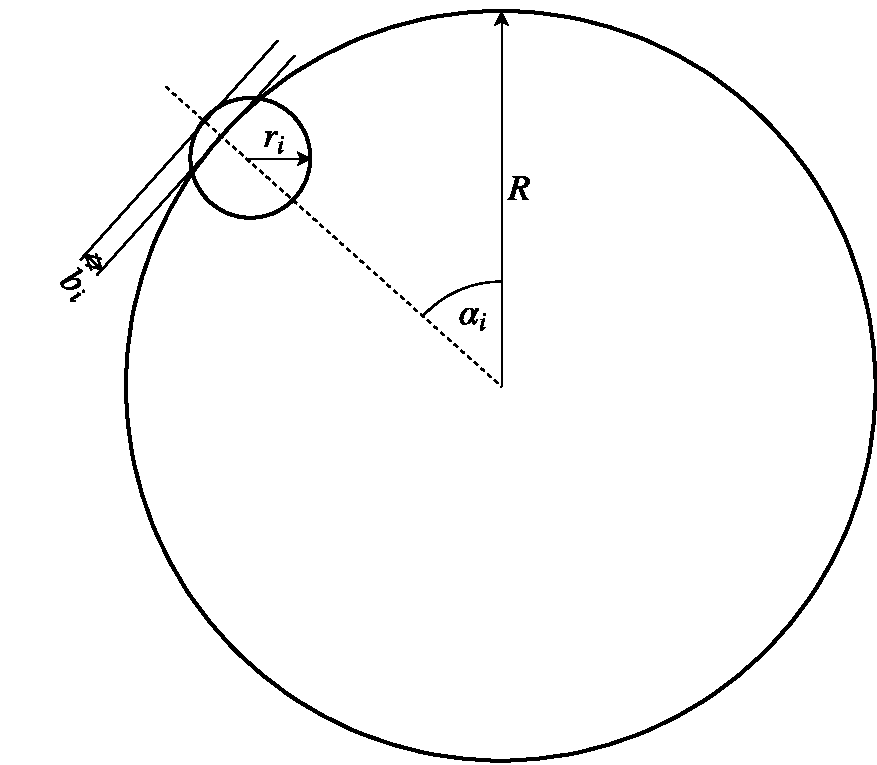
\includegraphics[width=0.38\linewidth]{rod_model-front_view.pdf}
\captionsetup{width=.7\linewidth}
\caption{A front-to-back view of an example of a rod model with one patch. In a configuration file, $R$
corresponds to the \texttt{rod\_radius} parameter and $\alpha_i$, $r_i$ and $b_i$ correspond to the
$i^\text{th}$ elements of the \texttt{patch\_angles}, \texttt{patch\_bead\_radii} and
\texttt{patch\_bulge\_out} tuples.}
\label{img:rod_front}
\end{figure}

\begin{figure}[!h]
\centering
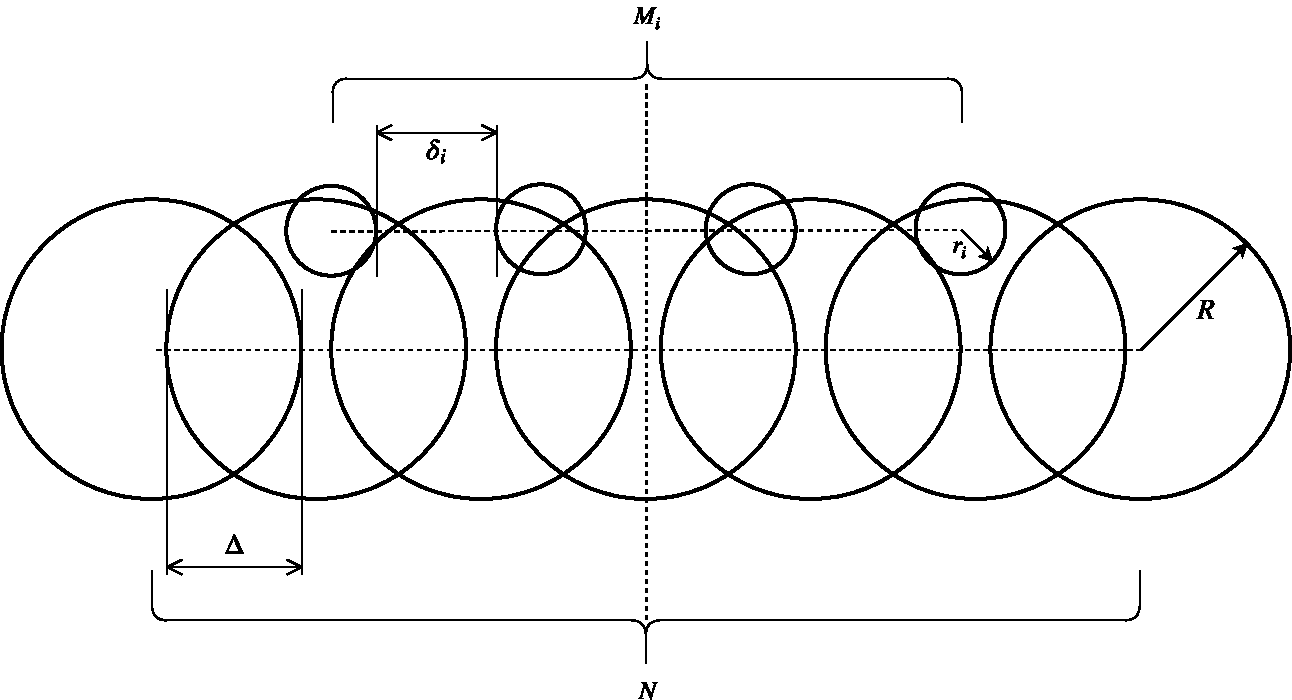
\includegraphics[width=0.7\linewidth]{rod_model-side_view.pdf}
\captionsetup{width=.7\linewidth}
\caption{A side view of an example of a rod model with one patch. In the library, $\Delta$ (the overlap
between body beads) is calculated from the \texttt{rod\_length} (from tip to tip) and
\texttt{rod\_radius} ($R$) parameters and the number of body beads $N$, which is implicitly given with
the \texttt{state\_structures} parameter; $\delta_i$ (the distance between interaction sites
in a patch) corresponds to the $i^\text{th}$ element of the \texttt{patch\_bead\_sep} tuple in the
configuration file.}
\label{img:rod_side}
\end{figure}

\vspace{1em}

Some of the features and restrictions of the model are:
\begin{itemize}
	\item The number of body beads, patches and beads in each of the patches are also set in the
	configuration file, although implicitly through the \texttt{state\_structures} parameter that also
	defines the types of all the beads in each of the states;
	\item All states have to have the same geometry (numbers and positions of beads), but some of them can
	be made \emph{inactive} (e.g. 0 interaction strength, or just volume exclusion) in some states;
	\item The parameters of an interaction are its \textbf{type} (i.e. potential function),
	\textbf{strength} and \textbf{range}, and are given separately for each pair of bead types. The
	\textbf{range} of an interaction is taken to be the distance between the \emph{surfaces} of two beads at
	which the interaction vanishes, where the \emph{surface} of a bead is taken to be the radius distance
	from its center/location.
\end{itemize}

\subsection{Running a simulation}

This library is written in Python 2.7 and uses the Python wrapper of the LAMMPS library interface to
communicate with the LAMMPS program. In order to use it the user first has to make a Python script that
imports the \texttt{lammps} module and create an instance of \texttt{Lammps} (or \texttt{PyLammps})
which they will afterwards use in essentially the same way as in a standard textual input script.
Secondly, the user has to construct a \texttt{Rod\_model} object using the model configuration file they
previously defined. This object holds all data from the configuration file and a lot of additional,
inferred ones that instances of the \texttt{Simulation} class use, but can also come in handy to the
user. These two objects (a \texttt{Lammps} and a \texttt{Rod\_model} instance) can then be used to make
a \texttt{Simulation} object.

\vspace{1em}

The idea of the library is for it to be used to create and manipulate the (states of the) rods as
independently as possible of any other particles or features in LAMMPS. To this end a
\texttt{Simulation} object needs to be instantiated and \texttt{setup} with some information about all
the other LAMMPS elements (particles, interactions, etc.) that are or will be used in the simulation.
After that the object's methods (e.g. \texttt{create\_rods}, \texttt{set\_rod\_dynamics},
\texttt{state\_change\_MC}) can be used to create rods, set their dynamics and manipulate their states.
In the meanwhile LAMMPS can be used normally (through Python) to manipulate in any which way any other
particles or properties of the system.

\vspace{1em}

A demonstration of all of this and an example of how the library can be used can be found in the
\texttt{examples} directory in the form of a console application (simulate\_nvt.py).

\subsubsection*{Technical limitations and development points}

\begin{enumerate}
	\item It is impossible to delete rods after they are created \label{enum:1};
	\item Consequently to \ref{enum:1}., a grand-canonical ensemble cannot be established (\texttt{fix
	gcmc} can't be used) for any of the rod states. However, a near-constant density of rods in a certain
	state might be achieved by simply adding new rods in that state (if that state gets depleted during the
	simulation);
	\item Currently MPI functionality is not available, a simulation with rods can only be run on a single
	core (this is probably fixable without major changes to the library);
	\item Energy minimization algorithms from LAMMPS cannot be used on the rods because they are defined as
	rigid objects. This makes random initial configurations hard to generate.
\end{enumerate}

\end{document}
